\documentclass[]{article}
\usepackage{lmodern}
\usepackage{amssymb,amsmath}
\usepackage{ifxetex,ifluatex}
\usepackage{fixltx2e} % provides \textsubscript
\ifnum 0\ifxetex 1\fi\ifluatex 1\fi=0 % if pdftex
  \usepackage[T1]{fontenc}
  \usepackage[utf8]{inputenc}
\else % if luatex or xelatex
  \ifxetex
    \usepackage{mathspec}
  \else
    \usepackage{fontspec}
  \fi
  \defaultfontfeatures{Ligatures=TeX,Scale=MatchLowercase}
\fi
% use upquote if available, for straight quotes in verbatim environments
\IfFileExists{upquote.sty}{\usepackage{upquote}}{}
% use microtype if available
\IfFileExists{microtype.sty}{%
\usepackage{microtype}
\UseMicrotypeSet[protrusion]{basicmath} % disable protrusion for tt fonts
}{}
\usepackage[margin=1in]{geometry}
\usepackage{hyperref}
\hypersetup{unicode=true,
            pdftitle={R Notebook},
            pdfborder={0 0 0},
            breaklinks=true}
\urlstyle{same}  % don't use monospace font for urls
\usepackage{color}
\usepackage{fancyvrb}
\newcommand{\VerbBar}{|}
\newcommand{\VERB}{\Verb[commandchars=\\\{\}]}
\DefineVerbatimEnvironment{Highlighting}{Verbatim}{commandchars=\\\{\}}
% Add ',fontsize=\small' for more characters per line
\usepackage{framed}
\definecolor{shadecolor}{RGB}{248,248,248}
\newenvironment{Shaded}{\begin{snugshade}}{\end{snugshade}}
\newcommand{\KeywordTok}[1]{\textcolor[rgb]{0.13,0.29,0.53}{\textbf{{#1}}}}
\newcommand{\DataTypeTok}[1]{\textcolor[rgb]{0.13,0.29,0.53}{{#1}}}
\newcommand{\DecValTok}[1]{\textcolor[rgb]{0.00,0.00,0.81}{{#1}}}
\newcommand{\BaseNTok}[1]{\textcolor[rgb]{0.00,0.00,0.81}{{#1}}}
\newcommand{\FloatTok}[1]{\textcolor[rgb]{0.00,0.00,0.81}{{#1}}}
\newcommand{\ConstantTok}[1]{\textcolor[rgb]{0.00,0.00,0.00}{{#1}}}
\newcommand{\CharTok}[1]{\textcolor[rgb]{0.31,0.60,0.02}{{#1}}}
\newcommand{\SpecialCharTok}[1]{\textcolor[rgb]{0.00,0.00,0.00}{{#1}}}
\newcommand{\StringTok}[1]{\textcolor[rgb]{0.31,0.60,0.02}{{#1}}}
\newcommand{\VerbatimStringTok}[1]{\textcolor[rgb]{0.31,0.60,0.02}{{#1}}}
\newcommand{\SpecialStringTok}[1]{\textcolor[rgb]{0.31,0.60,0.02}{{#1}}}
\newcommand{\ImportTok}[1]{{#1}}
\newcommand{\CommentTok}[1]{\textcolor[rgb]{0.56,0.35,0.01}{\textit{{#1}}}}
\newcommand{\DocumentationTok}[1]{\textcolor[rgb]{0.56,0.35,0.01}{\textbf{\textit{{#1}}}}}
\newcommand{\AnnotationTok}[1]{\textcolor[rgb]{0.56,0.35,0.01}{\textbf{\textit{{#1}}}}}
\newcommand{\CommentVarTok}[1]{\textcolor[rgb]{0.56,0.35,0.01}{\textbf{\textit{{#1}}}}}
\newcommand{\OtherTok}[1]{\textcolor[rgb]{0.56,0.35,0.01}{{#1}}}
\newcommand{\FunctionTok}[1]{\textcolor[rgb]{0.00,0.00,0.00}{{#1}}}
\newcommand{\VariableTok}[1]{\textcolor[rgb]{0.00,0.00,0.00}{{#1}}}
\newcommand{\ControlFlowTok}[1]{\textcolor[rgb]{0.13,0.29,0.53}{\textbf{{#1}}}}
\newcommand{\OperatorTok}[1]{\textcolor[rgb]{0.81,0.36,0.00}{\textbf{{#1}}}}
\newcommand{\BuiltInTok}[1]{{#1}}
\newcommand{\ExtensionTok}[1]{{#1}}
\newcommand{\PreprocessorTok}[1]{\textcolor[rgb]{0.56,0.35,0.01}{\textit{{#1}}}}
\newcommand{\AttributeTok}[1]{\textcolor[rgb]{0.77,0.63,0.00}{{#1}}}
\newcommand{\RegionMarkerTok}[1]{{#1}}
\newcommand{\InformationTok}[1]{\textcolor[rgb]{0.56,0.35,0.01}{\textbf{\textit{{#1}}}}}
\newcommand{\WarningTok}[1]{\textcolor[rgb]{0.56,0.35,0.01}{\textbf{\textit{{#1}}}}}
\newcommand{\AlertTok}[1]{\textcolor[rgb]{0.94,0.16,0.16}{{#1}}}
\newcommand{\ErrorTok}[1]{\textcolor[rgb]{0.64,0.00,0.00}{\textbf{{#1}}}}
\newcommand{\NormalTok}[1]{{#1}}
\usepackage{graphicx,grffile}
\makeatletter
\def\maxwidth{\ifdim\Gin@nat@width>\linewidth\linewidth\else\Gin@nat@width\fi}
\def\maxheight{\ifdim\Gin@nat@height>\textheight\textheight\else\Gin@nat@height\fi}
\makeatother
% Scale images if necessary, so that they will not overflow the page
% margins by default, and it is still possible to overwrite the defaults
% using explicit options in \includegraphics[width, height, ...]{}
\setkeys{Gin}{width=\maxwidth,height=\maxheight,keepaspectratio}
\IfFileExists{parskip.sty}{%
\usepackage{parskip}
}{% else
\setlength{\parindent}{0pt}
\setlength{\parskip}{6pt plus 2pt minus 1pt}
}
\setlength{\emergencystretch}{3em}  % prevent overfull lines
\providecommand{\tightlist}{%
  \setlength{\itemsep}{0pt}\setlength{\parskip}{0pt}}
\setcounter{secnumdepth}{0}
% Redefines (sub)paragraphs to behave more like sections
\ifx\paragraph\undefined\else
\let\oldparagraph\paragraph
\renewcommand{\paragraph}[1]{\oldparagraph{#1}\mbox{}}
\fi
\ifx\subparagraph\undefined\else
\let\oldsubparagraph\subparagraph
\renewcommand{\subparagraph}[1]{\oldsubparagraph{#1}\mbox{}}
\fi

%%% Use protect on footnotes to avoid problems with footnotes in titles
\let\rmarkdownfootnote\footnote%
\def\footnote{\protect\rmarkdownfootnote}

%%% Change title format to be more compact
\usepackage{titling}

% Create subtitle command for use in maketitle
\newcommand{\subtitle}[1]{
  \posttitle{
    \begin{center}\large#1\end{center}
    }
}

\setlength{\droptitle}{-2em}
  \title{R Notebook}
  \pretitle{\vspace{\droptitle}\centering\huge}
  \posttitle{\par}
  \author{}
  \preauthor{}\postauthor{}
  \date{}
  \predate{}\postdate{}


\begin{document}
\maketitle

This is an \href{http://rmarkdown.rstudio.com}{R Markdown} Notebook.
When you execute code within the notebook, the results appear beneath
the code.

Try executing this chunk by clicking the \emph{Run} button within the
chunk or by placing your cursor inside it and pressing
\emph{Ctrl+Shift+Enter}.

\begin{Shaded}
\begin{Highlighting}[]
\NormalTok{oj <-}\StringTok{ }\KeywordTok{read.table}\NormalTok{(}\StringTok{"oj.csv"}\NormalTok{,}\DataTypeTok{header=}\OtherTok{TRUE}\NormalTok{,}\DataTypeTok{sep=}\StringTok{","}\NormalTok{)}
\KeywordTok{library}\NormalTok{(lattice)}
\KeywordTok{par}\NormalTok{(}\DataTypeTok{mfrow =} \KeywordTok{c}\NormalTok{(}\DecValTok{2}\NormalTok{,}\DecValTok{2}\NormalTok{))}
\NormalTok{df <-}\StringTok{ }\KeywordTok{unique}\NormalTok{(oj[}\KeywordTok{c}\NormalTok{(}\DecValTok{1}\NormalTok{,}\DecValTok{7}\NormalTok{:}\DecValTok{17}\NormalTok{)]) }
\NormalTok{var_list<-}\StringTok{ }\KeywordTok{names}\NormalTok{(df)[}\DecValTok{2}\NormalTok{:}\DecValTok{12}\NormalTok{]}
\NormalTok{models <-}\StringTok{ }\KeywordTok{lapply}\NormalTok{(var_list, }
          \NormalTok{function(x) }
            \NormalTok{\{}
             \NormalTok{mod =}\StringTok{ }\KeywordTok{lm}\NormalTok{(}\KeywordTok{substitute}\NormalTok{(store ~}\StringTok{ }\NormalTok{i, }\KeywordTok{list}\NormalTok{(}\DataTypeTok{i =} \KeywordTok{as.name}\NormalTok{(x))), }\DataTypeTok{data =} \NormalTok{df)}
            \NormalTok{\})}
\KeywordTok{par}\NormalTok{(}\DataTypeTok{mfrow =} \KeywordTok{c}\NormalTok{(}\DecValTok{2}\NormalTok{,}\DecValTok{2}\NormalTok{))}
\KeywordTok{invisible}\NormalTok{(}\KeywordTok{lapply}\NormalTok{(models,plot))}
\end{Highlighting}
\end{Shaded}

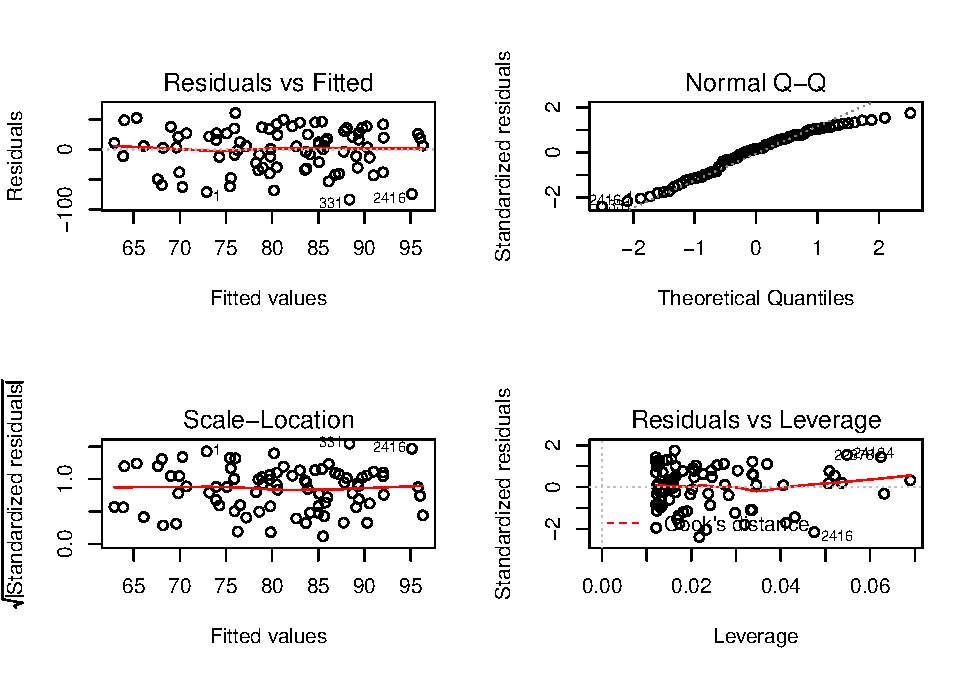
\includegraphics{Desc_stats_files/figure-latex/unnamed-chunk-1-1.pdf}
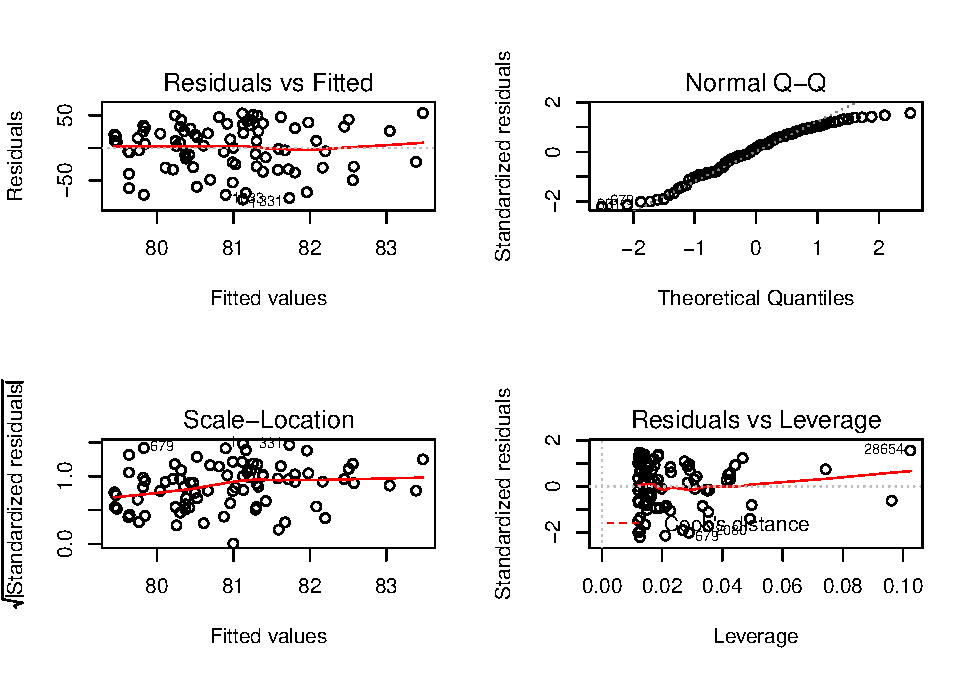
\includegraphics{Desc_stats_files/figure-latex/unnamed-chunk-1-2.pdf}
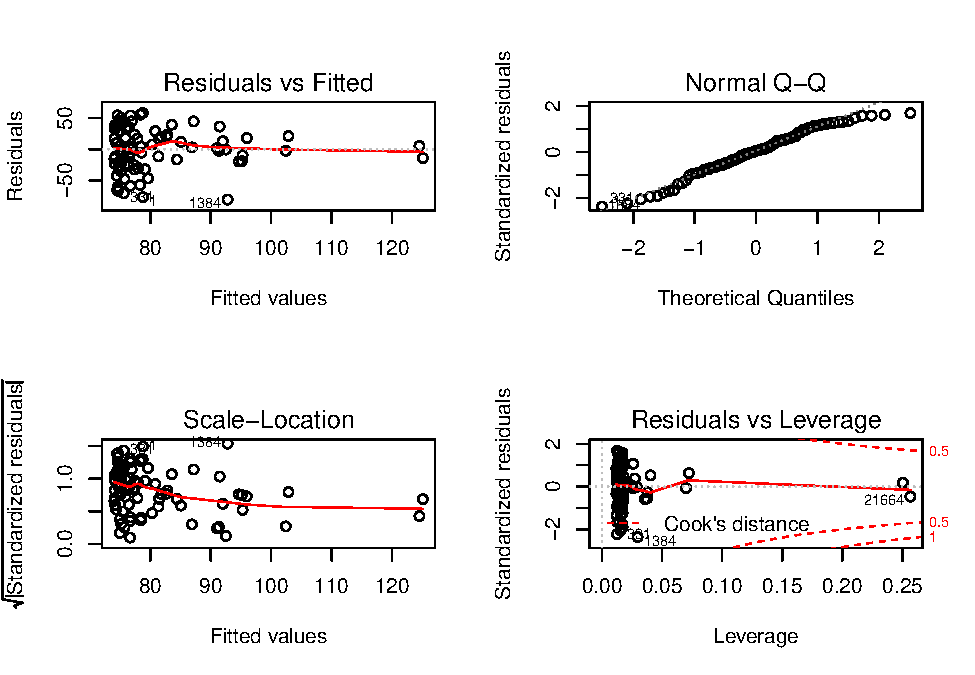
\includegraphics{Desc_stats_files/figure-latex/unnamed-chunk-1-3.pdf}
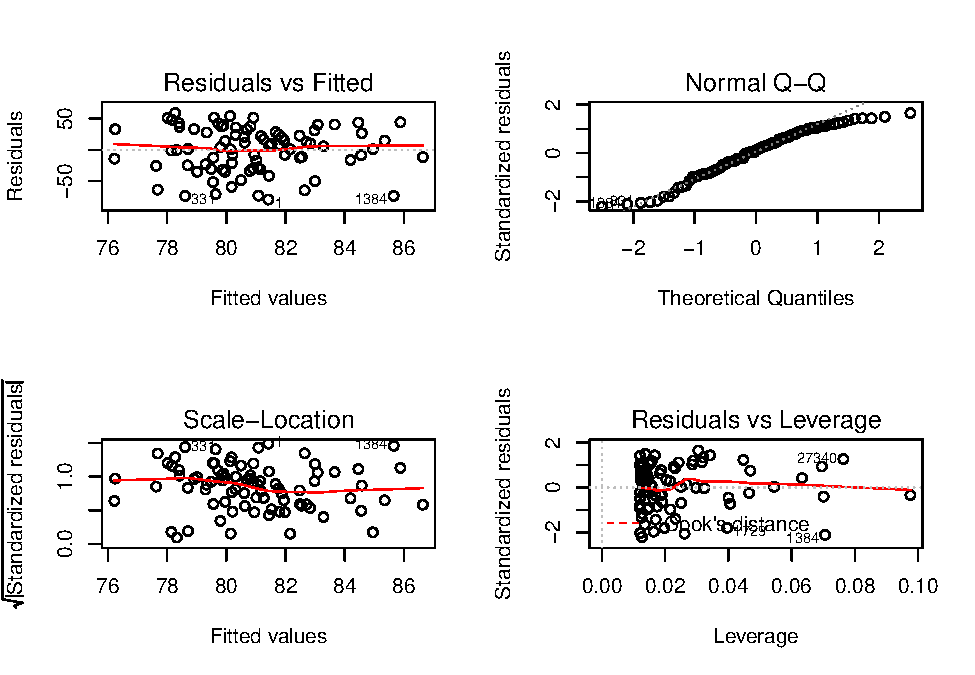
\includegraphics{Desc_stats_files/figure-latex/unnamed-chunk-1-4.pdf}
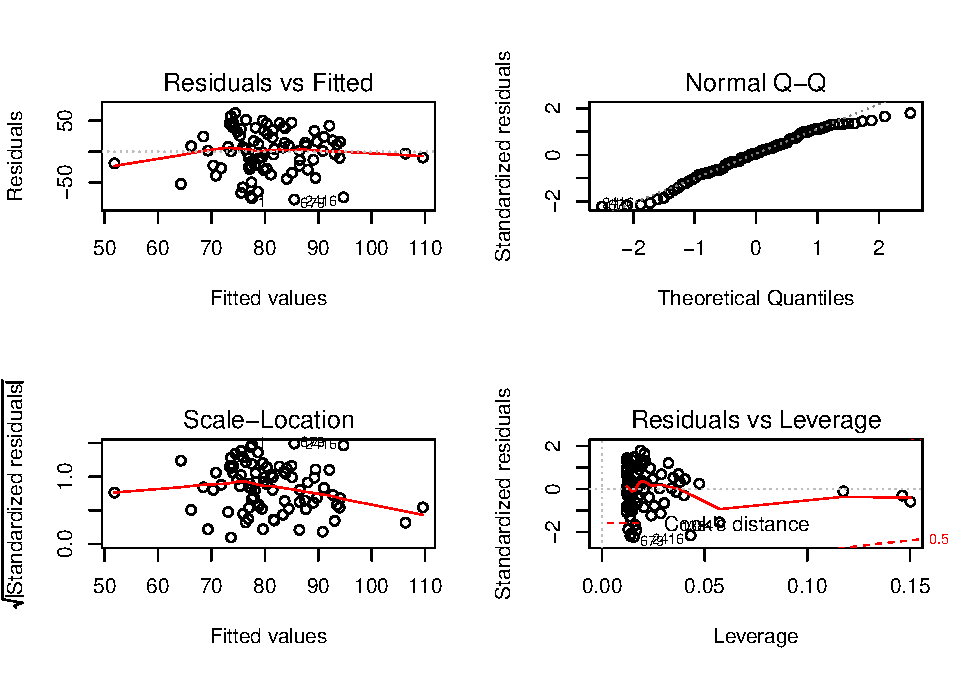
\includegraphics{Desc_stats_files/figure-latex/unnamed-chunk-1-5.pdf}
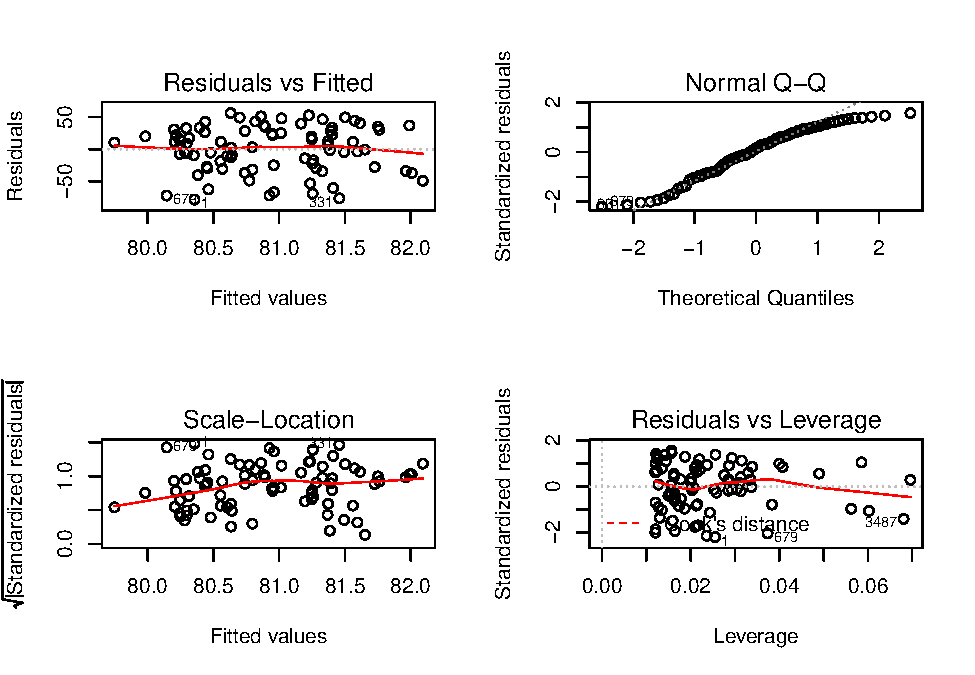
\includegraphics{Desc_stats_files/figure-latex/unnamed-chunk-1-6.pdf}
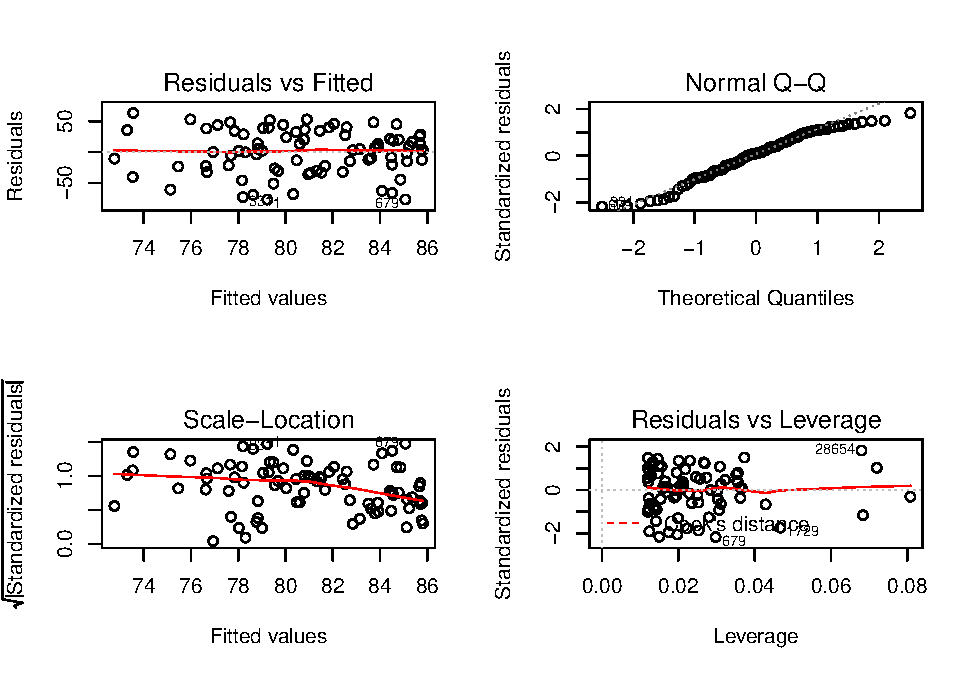
\includegraphics{Desc_stats_files/figure-latex/unnamed-chunk-1-7.pdf}
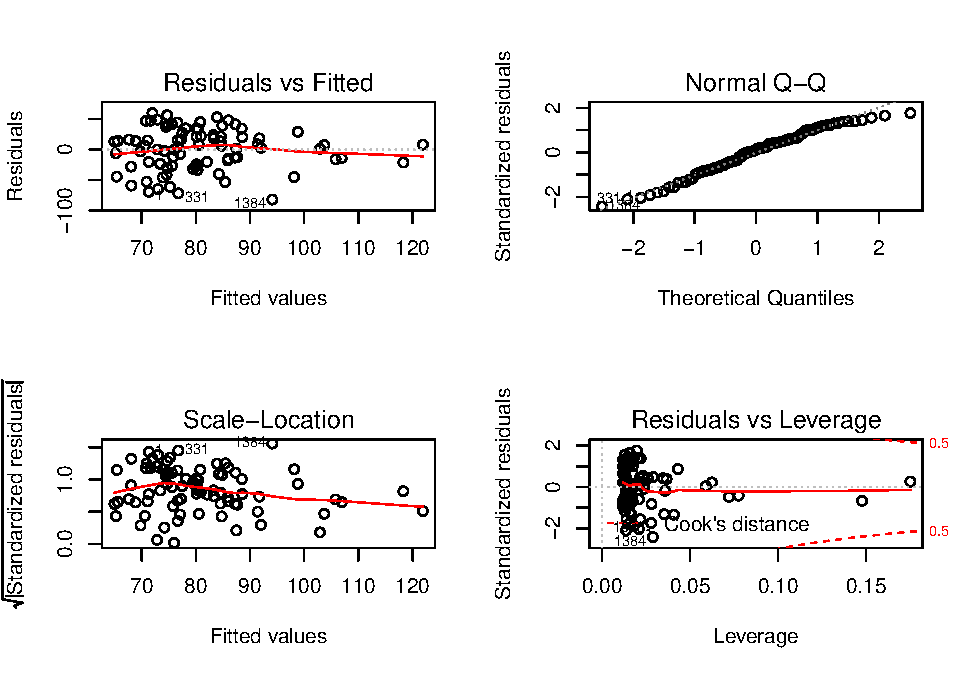
\includegraphics{Desc_stats_files/figure-latex/unnamed-chunk-1-8.pdf}
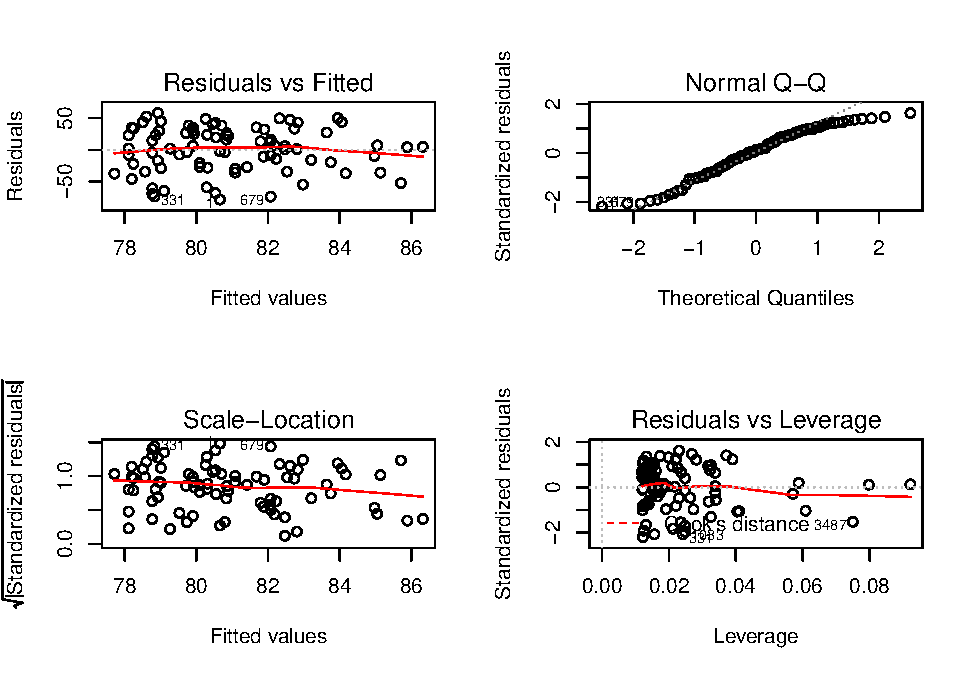
\includegraphics{Desc_stats_files/figure-latex/unnamed-chunk-1-9.pdf}
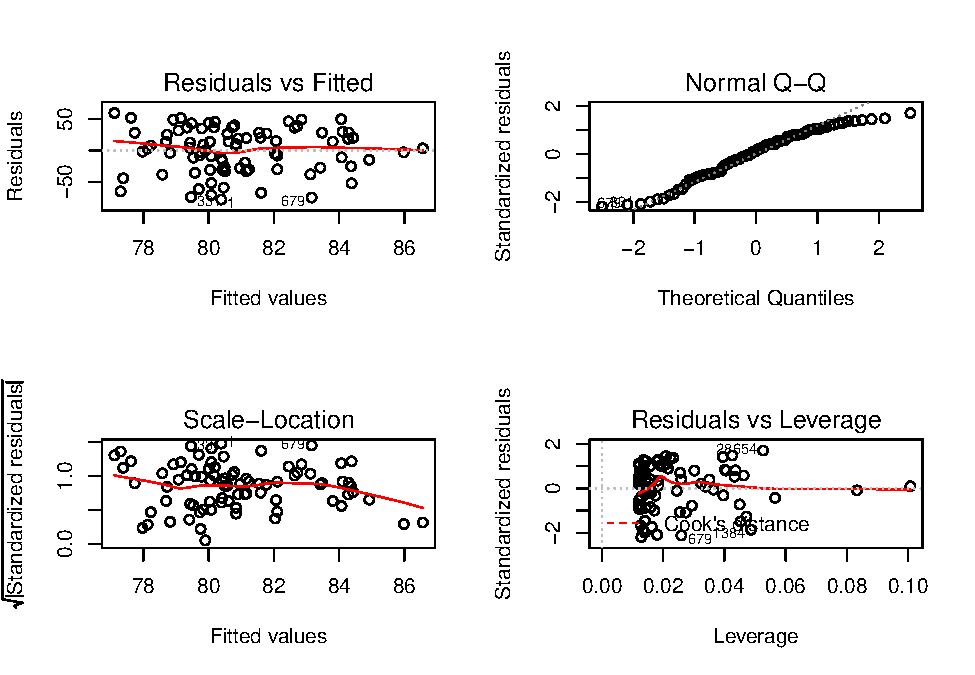
\includegraphics{Desc_stats_files/figure-latex/unnamed-chunk-1-10.pdf}
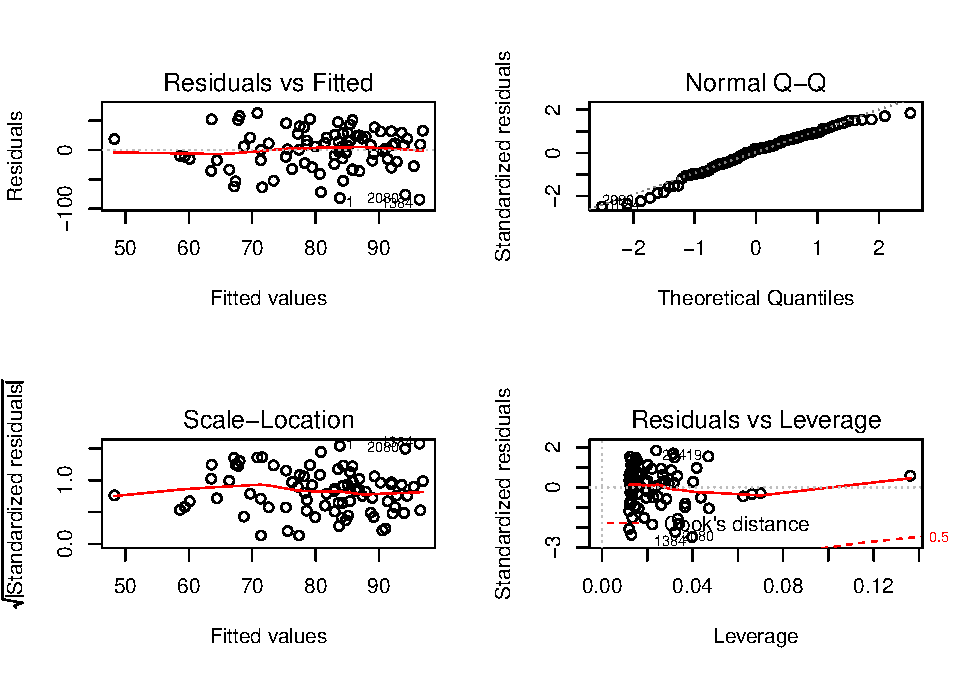
\includegraphics{Desc_stats_files/figure-latex/unnamed-chunk-1-11.pdf}

\begin{Shaded}
\begin{Highlighting}[]
\KeywordTok{library}\NormalTok{(ggplot2)}
\end{Highlighting}
\end{Shaded}

\begin{verbatim}
## Warning: package 'ggplot2' was built under R version 3.3.2
\end{verbatim}

\begin{Shaded}
\begin{Highlighting}[]
\NormalTok{df <-}\StringTok{ }\KeywordTok{unique}\NormalTok{(oj[}\KeywordTok{c}\NormalTok{(}\DecValTok{1}\NormalTok{,}\DecValTok{7}\NormalTok{:}\DecValTok{17}\NormalTok{)]) }
\NormalTok{var_list<-}\StringTok{ }\KeywordTok{names}\NormalTok{(df)[}\DecValTok{2}\NormalTok{:}\DecValTok{12}\NormalTok{]}
\NormalTok{plots <-}\StringTok{ }\NormalTok{function(i)\{}
                     \KeywordTok{ggplot}\NormalTok{(df, }\KeywordTok{aes}\NormalTok{(}\DataTypeTok{x =} \NormalTok{df[i])) +}\StringTok{ }
\StringTok{                     }\KeywordTok{geom_histogram}\NormalTok{(}\KeywordTok{aes}\NormalTok{(}\DataTypeTok{y =} \NormalTok{..density..),}\DataTypeTok{colour =} \StringTok{"black"}\NormalTok{, }
                                    \DataTypeTok{fill =} \StringTok{"yellow"}\NormalTok{,}\DataTypeTok{binwidth =} \FloatTok{0.02}\NormalTok{) +}
\StringTok{                     }\KeywordTok{geom_density}\NormalTok{(}\DataTypeTok{alpha =} \FloatTok{0.2}\NormalTok{, }\DataTypeTok{fill =} \StringTok{"blue"}\NormalTok{,}\DataTypeTok{linetype =} \StringTok{"dashed"}\NormalTok{) +}\StringTok{ }
\StringTok{                     }\KeywordTok{geom_vline}\NormalTok{(}\KeywordTok{aes}\NormalTok{(}\DataTypeTok{xintercept=}\KeywordTok{mean}\NormalTok{(df[i], }\DataTypeTok{na.rm =} \OtherTok{TRUE}\NormalTok{)),}
                                \DataTypeTok{color =} \StringTok{"black"}\NormalTok{,}\DataTypeTok{linetype =} \StringTok{"dashed"}\NormalTok{, }\DataTypeTok{size =} \DecValTok{1}\NormalTok{) +}
\StringTok{                     }\KeywordTok{xlab}\NormalTok{(}\KeywordTok{names}\NormalTok{(df)[i]) +}
\StringTok{                     }\KeywordTok{ggtitle}\NormalTok{(}\KeywordTok{paste}\NormalTok{(}\StringTok{"Histogram plot of "}\NormalTok{,}\KeywordTok{names}\NormalTok{(df)[i]))\}}
\KeywordTok{par}\NormalTok{(}\DataTypeTok{mfrow =} \KeywordTok{c}\NormalTok{(}\DecValTok{2}\NormalTok{,}\DecValTok{2}\NormalTok{))}
\KeywordTok{lapply}\NormalTok{(}\DecValTok{2}\NormalTok{:}\DecValTok{12}\NormalTok{,}\DataTypeTok{FUN =} \NormalTok{plots)}
\end{Highlighting}
\end{Shaded}

\begin{verbatim}
## [[1]]
\end{verbatim}

\begin{verbatim}
## Don't know how to automatically pick scale for object of type data.frame. Defaulting to continuous.
\end{verbatim}

\begin{verbatim}
## Warning in mean.default(df[i], na.rm = TRUE): argument is not numeric or
## logical: returning NA
\end{verbatim}

\begin{verbatim}
## Warning: Removed 83 rows containing missing values (geom_vline).
\end{verbatim}

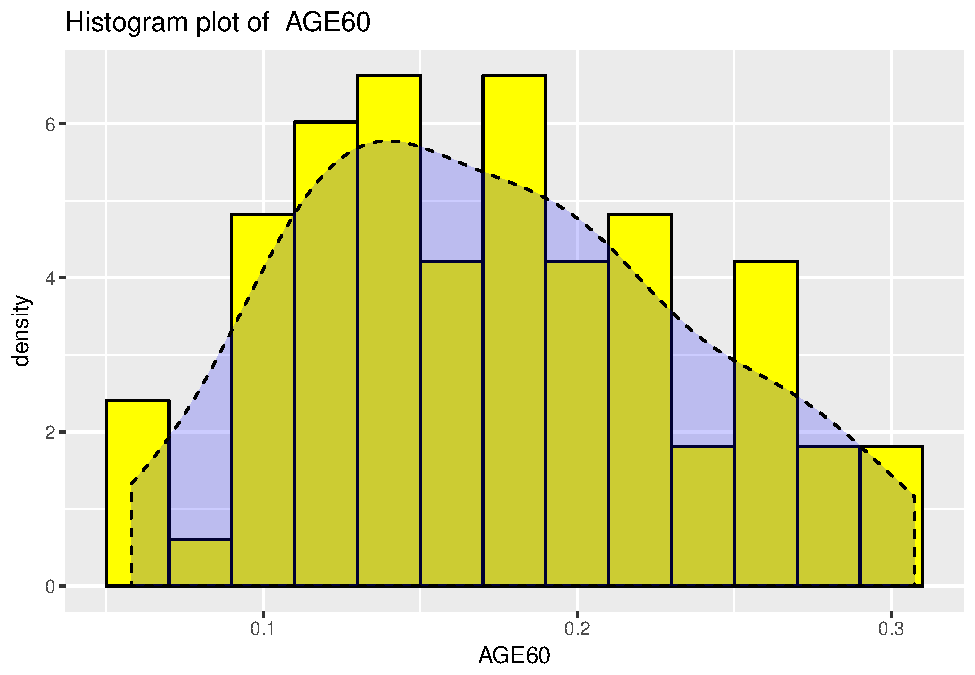
\includegraphics{Desc_stats_files/figure-latex/unnamed-chunk-2-1.pdf}

\begin{verbatim}
## 
## [[2]]
\end{verbatim}

\begin{verbatim}
## Don't know how to automatically pick scale for object of type data.frame. Defaulting to continuous.
\end{verbatim}

\begin{verbatim}
## Warning in mean.default(df[i], na.rm = TRUE): argument is not numeric or
## logical: returning NA

## Warning in mean.default(df[i], na.rm = TRUE): Removed 83 rows containing
## missing values (geom_vline).
\end{verbatim}

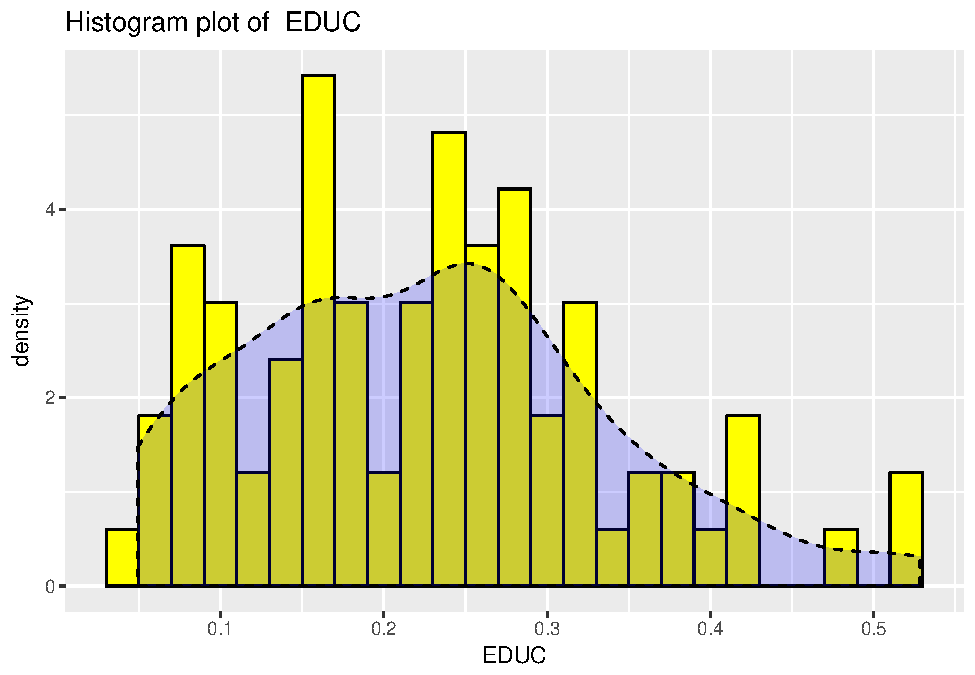
\includegraphics{Desc_stats_files/figure-latex/unnamed-chunk-2-2.pdf}

\begin{verbatim}
## 
## [[3]]
\end{verbatim}

\begin{verbatim}
## Don't know how to automatically pick scale for object of type data.frame. Defaulting to continuous.
\end{verbatim}

\begin{verbatim}
## Warning in mean.default(df[i], na.rm = TRUE): argument is not numeric or
## logical: returning NA

## Warning in mean.default(df[i], na.rm = TRUE): Removed 83 rows containing
## missing values (geom_vline).
\end{verbatim}

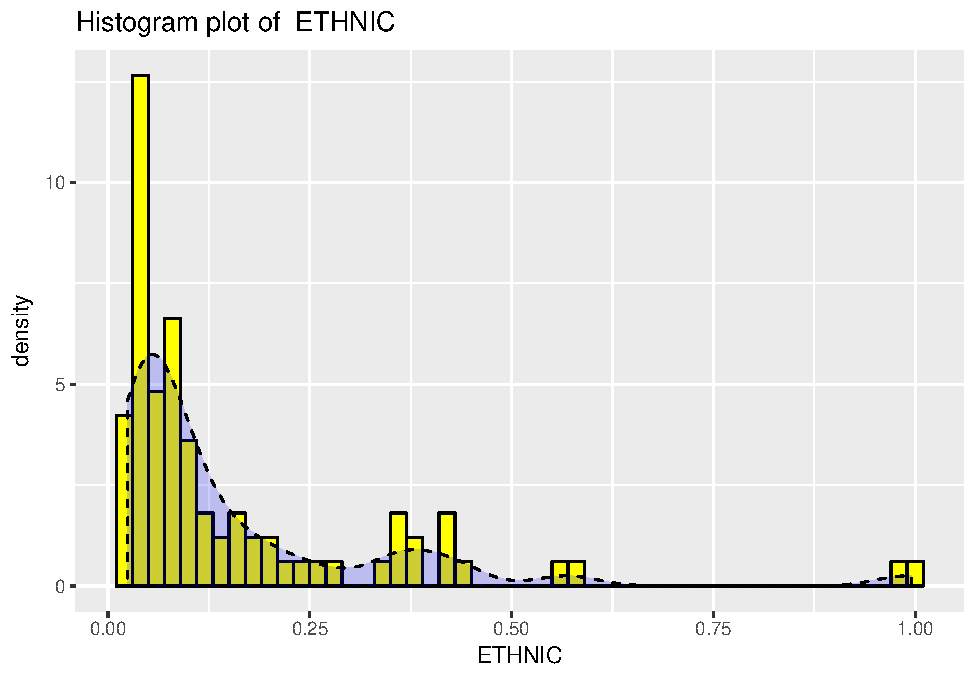
\includegraphics{Desc_stats_files/figure-latex/unnamed-chunk-2-3.pdf}

\begin{verbatim}
## 
## [[4]]
\end{verbatim}

\begin{verbatim}
## Don't know how to automatically pick scale for object of type data.frame. Defaulting to continuous.
\end{verbatim}

\begin{verbatim}
## Warning in mean.default(df[i], na.rm = TRUE): argument is not numeric or
## logical: returning NA

## Warning in mean.default(df[i], na.rm = TRUE): Removed 83 rows containing
## missing values (geom_vline).
\end{verbatim}

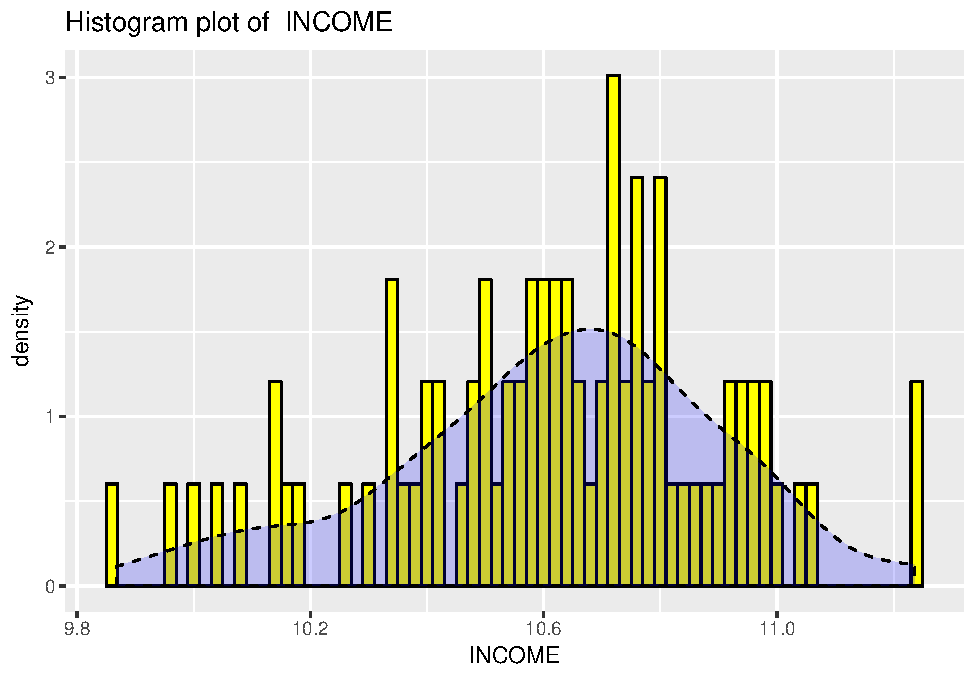
\includegraphics{Desc_stats_files/figure-latex/unnamed-chunk-2-4.pdf}

\begin{verbatim}
## 
## [[5]]
\end{verbatim}

\begin{verbatim}
## Don't know how to automatically pick scale for object of type data.frame. Defaulting to continuous.
\end{verbatim}

\begin{verbatim}
## Warning in mean.default(df[i], na.rm = TRUE): argument is not numeric or
## logical: returning NA

## Warning in mean.default(df[i], na.rm = TRUE): Removed 83 rows containing
## missing values (geom_vline).
\end{verbatim}

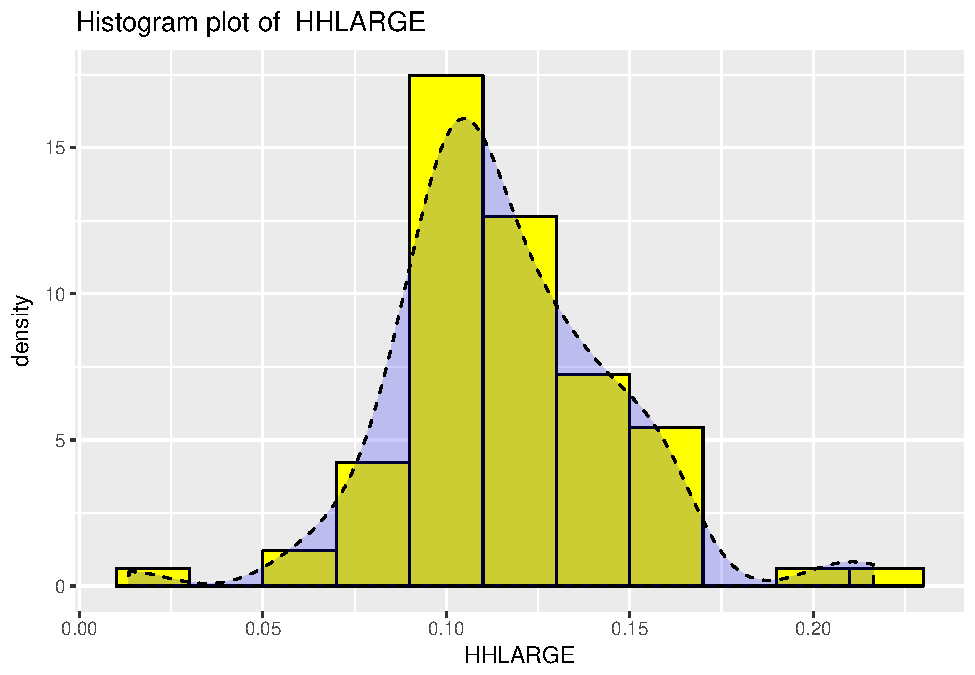
\includegraphics{Desc_stats_files/figure-latex/unnamed-chunk-2-5.pdf}

\begin{verbatim}
## 
## [[6]]
\end{verbatim}

\begin{verbatim}
## Don't know how to automatically pick scale for object of type data.frame. Defaulting to continuous.
\end{verbatim}

\begin{verbatim}
## Warning in mean.default(df[i], na.rm = TRUE): argument is not numeric or
## logical: returning NA

## Warning in mean.default(df[i], na.rm = TRUE): Removed 83 rows containing
## missing values (geom_vline).
\end{verbatim}

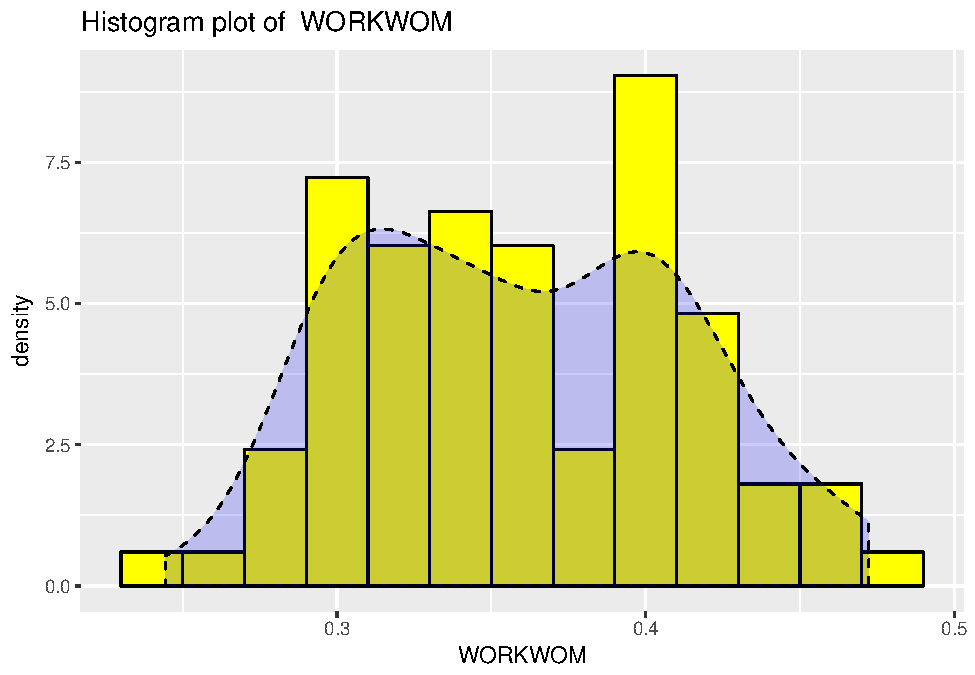
\includegraphics{Desc_stats_files/figure-latex/unnamed-chunk-2-6.pdf}

\begin{verbatim}
## 
## [[7]]
\end{verbatim}

\begin{verbatim}
## Don't know how to automatically pick scale for object of type data.frame. Defaulting to continuous.
\end{verbatim}

\begin{verbatim}
## Warning in mean.default(df[i], na.rm = TRUE): argument is not numeric or
## logical: returning NA

## Warning in mean.default(df[i], na.rm = TRUE): Removed 83 rows containing
## missing values (geom_vline).
\end{verbatim}

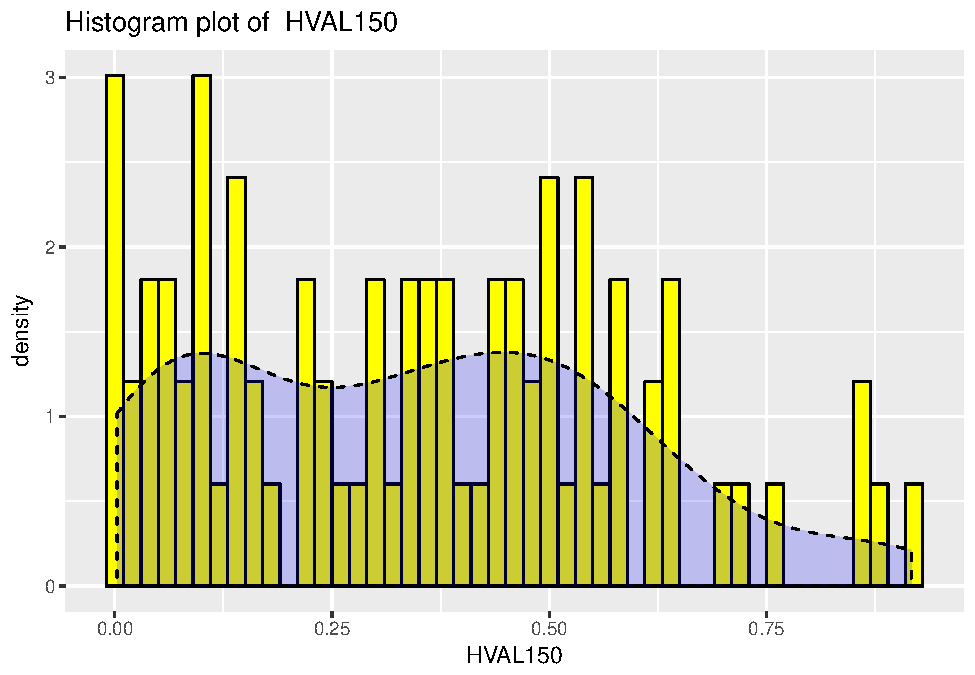
\includegraphics{Desc_stats_files/figure-latex/unnamed-chunk-2-7.pdf}

\begin{verbatim}
## 
## [[8]]
\end{verbatim}

\begin{verbatim}
## Don't know how to automatically pick scale for object of type data.frame. Defaulting to continuous.
\end{verbatim}

\begin{verbatim}
## Warning in mean.default(df[i], na.rm = TRUE): argument is not numeric or
## logical: returning NA

## Warning in mean.default(df[i], na.rm = TRUE): Removed 83 rows containing
## missing values (geom_vline).
\end{verbatim}

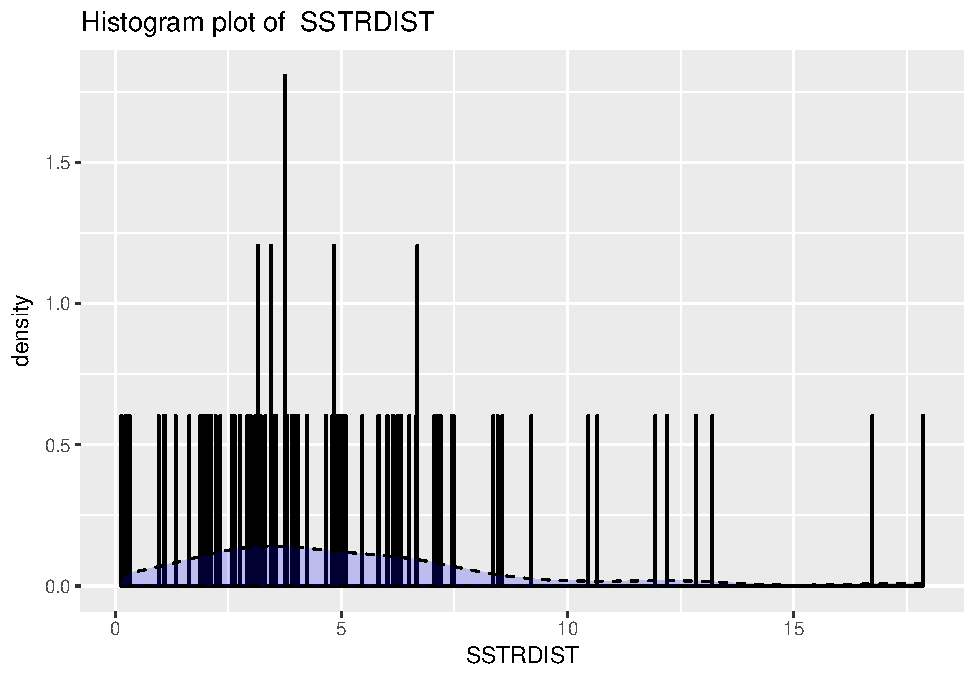
\includegraphics{Desc_stats_files/figure-latex/unnamed-chunk-2-8.pdf}

\begin{verbatim}
## 
## [[9]]
\end{verbatim}

\begin{verbatim}
## Don't know how to automatically pick scale for object of type data.frame. Defaulting to continuous.
\end{verbatim}

\begin{verbatim}
## Warning in mean.default(df[i], na.rm = TRUE): argument is not numeric or
## logical: returning NA

## Warning in mean.default(df[i], na.rm = TRUE): Removed 83 rows containing
## missing values (geom_vline).
\end{verbatim}

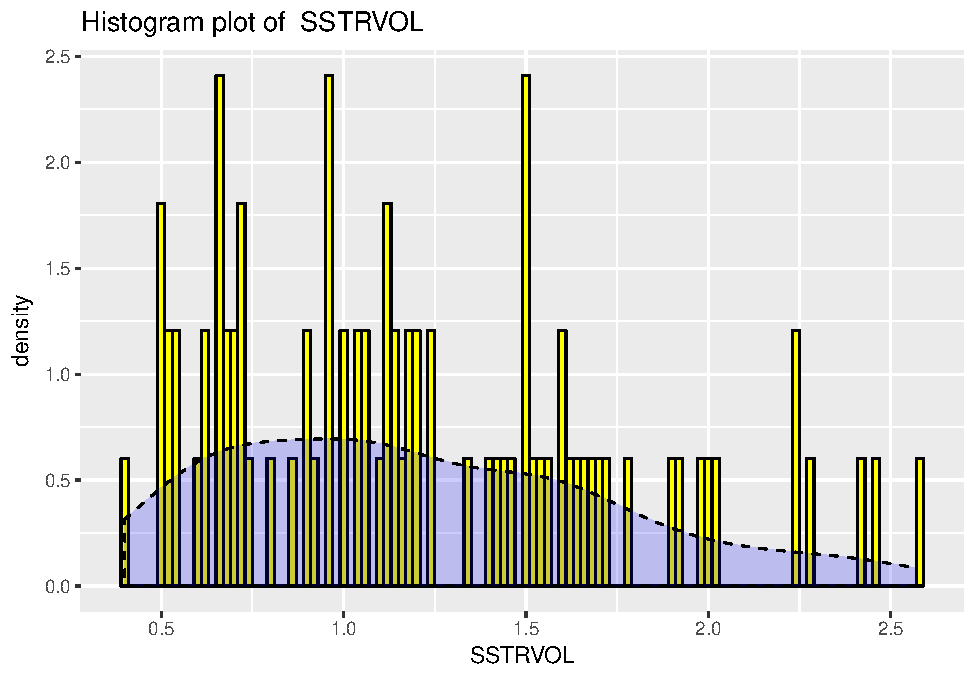
\includegraphics{Desc_stats_files/figure-latex/unnamed-chunk-2-9.pdf}

\begin{verbatim}
## 
## [[10]]
\end{verbatim}

\begin{verbatim}
## Don't know how to automatically pick scale for object of type data.frame. Defaulting to continuous.
\end{verbatim}

\begin{verbatim}
## Warning in mean.default(df[i], na.rm = TRUE): argument is not numeric or
## logical: returning NA

## Warning in mean.default(df[i], na.rm = TRUE): Removed 83 rows containing
## missing values (geom_vline).
\end{verbatim}

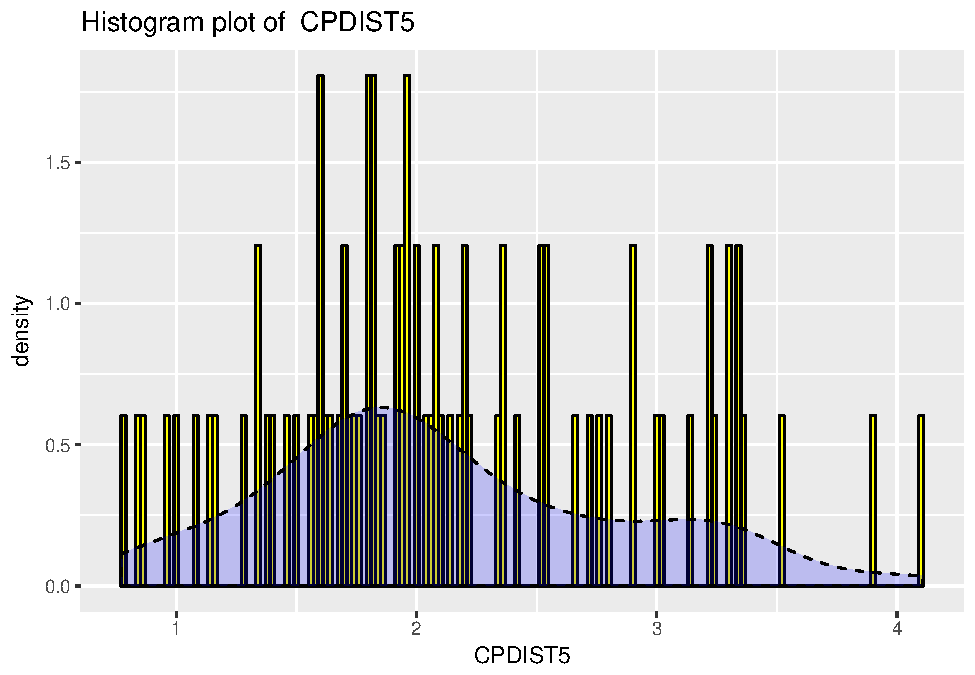
\includegraphics{Desc_stats_files/figure-latex/unnamed-chunk-2-10.pdf}

\begin{verbatim}
## 
## [[11]]
\end{verbatim}

\begin{verbatim}
## Don't know how to automatically pick scale for object of type data.frame. Defaulting to continuous.
\end{verbatim}

\begin{verbatim}
## Warning in mean.default(df[i], na.rm = TRUE): argument is not numeric or
## logical: returning NA

## Warning in mean.default(df[i], na.rm = TRUE): Removed 83 rows containing
## missing values (geom_vline).
\end{verbatim}

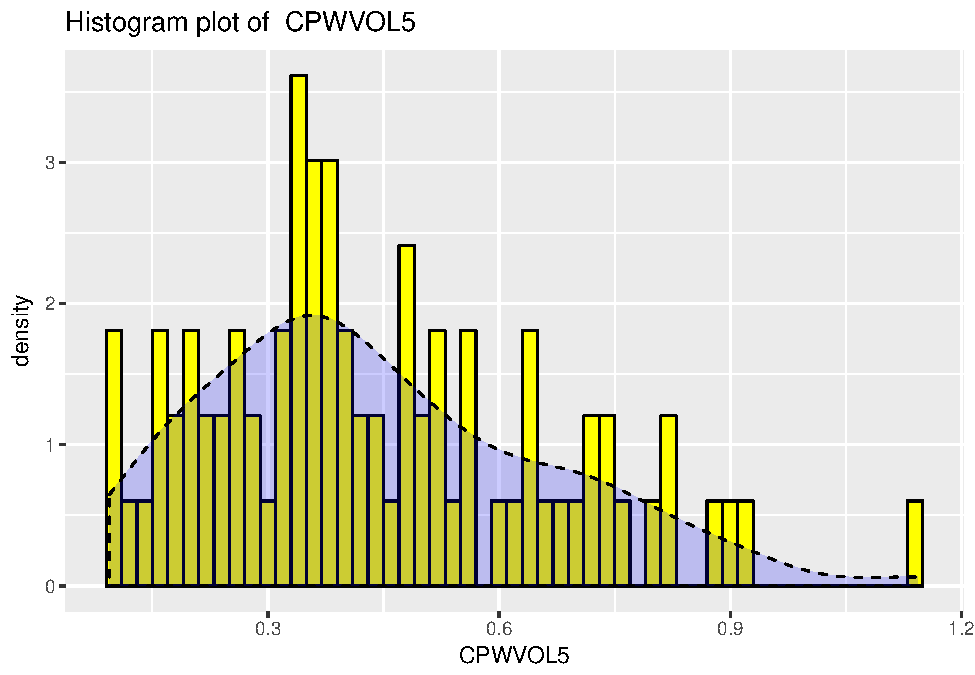
\includegraphics{Desc_stats_files/figure-latex/unnamed-chunk-2-11.pdf}

\begin{Shaded}
\begin{Highlighting}[]
\KeywordTok{library}\NormalTok{(s20x)}
\end{Highlighting}
\end{Shaded}

\begin{verbatim}
## Warning: package 's20x' was built under R version 3.3.2
\end{verbatim}

\begin{Shaded}
\begin{Highlighting}[]
\KeywordTok{pairs}\NormalTok{(df,}\DataTypeTok{col=}\StringTok{"green"}\NormalTok{,}\DataTypeTok{pch =} \DecValTok{20}\NormalTok{)}
\end{Highlighting}
\end{Shaded}

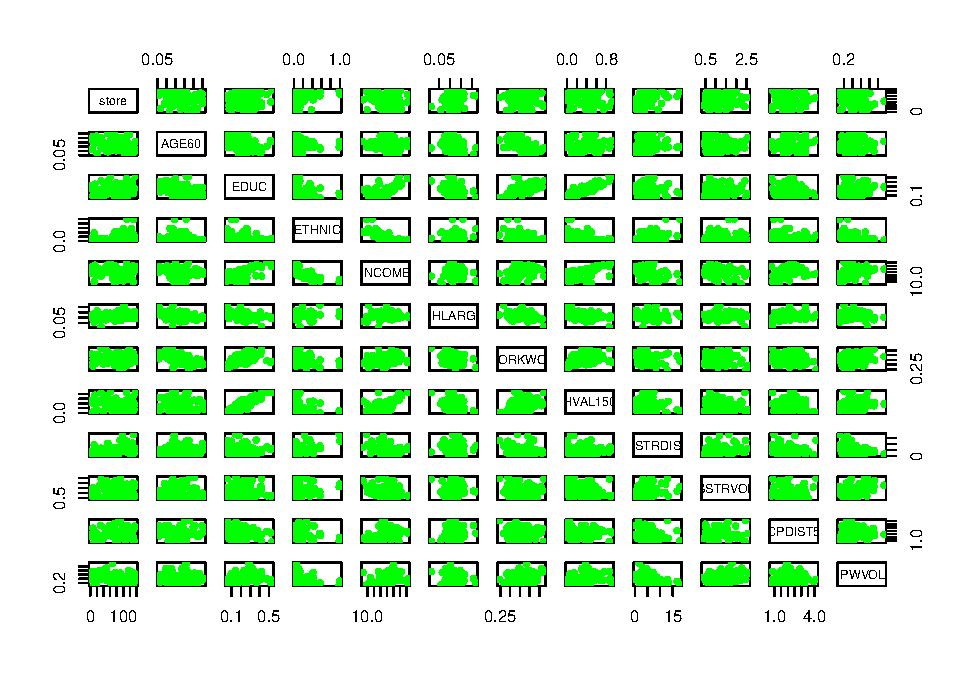
\includegraphics{Desc_stats_files/figure-latex/unnamed-chunk-3-1.pdf}

\begin{Shaded}
\begin{Highlighting}[]
\KeywordTok{pairs20x}\NormalTok{(df)}
\end{Highlighting}
\end{Shaded}

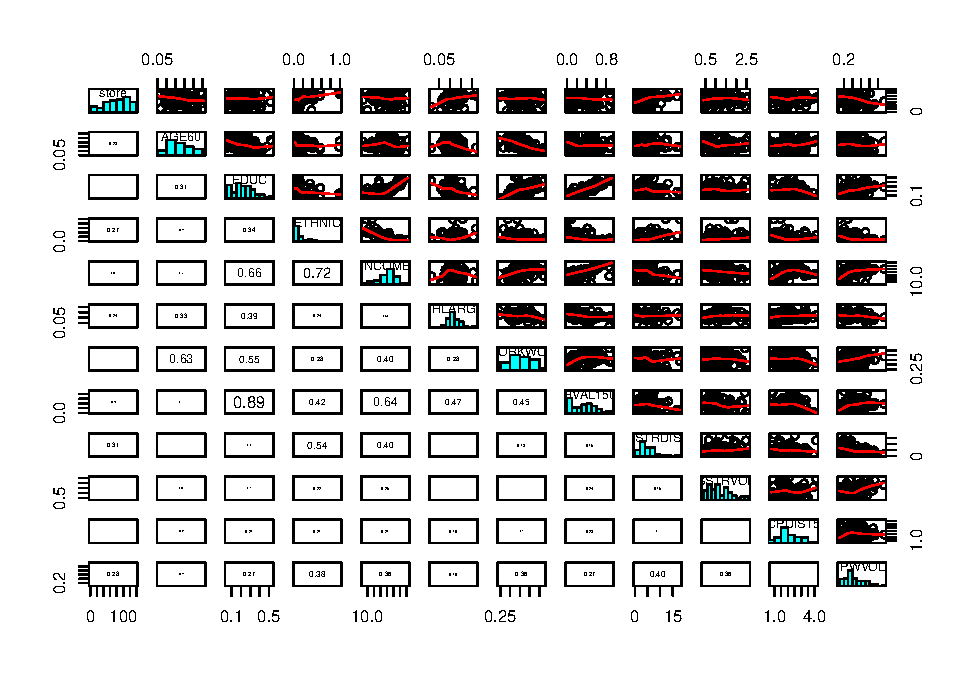
\includegraphics{Desc_stats_files/figure-latex/unnamed-chunk-3-2.pdf}

\begin{Shaded}
\begin{Highlighting}[]
\KeywordTok{library}\NormalTok{(stargazer)}
\end{Highlighting}
\end{Shaded}

\begin{verbatim}
## Warning: package 'stargazer' was built under R version 3.3.2
\end{verbatim}

\begin{verbatim}
## 
## Please cite as:
\end{verbatim}

\begin{verbatim}
##  Hlavac, Marek (2015). stargazer: Well-Formatted Regression and Summary Statistics Tables.
\end{verbatim}

\begin{verbatim}
##  R package version 5.2. http://CRAN.R-project.org/package=stargazer
\end{verbatim}

\begin{Shaded}
\begin{Highlighting}[]
\KeywordTok{library}\NormalTok{(doBy)}
\end{Highlighting}
\end{Shaded}

\begin{verbatim}
## Warning: package 'doBy' was built under R version 3.3.2
\end{verbatim}

\begin{Shaded}
\begin{Highlighting}[]
\KeywordTok{stargazer}\NormalTok{(df, }\DataTypeTok{type =} \StringTok{"text"}\NormalTok{, }\DataTypeTok{median =} \OtherTok{TRUE}\NormalTok{, }\DataTypeTok{digits =} \DecValTok{2}\NormalTok{)}
\end{Highlighting}
\end{Shaded}

\begin{verbatim}
## 
## ==============================================
## Statistic N  Mean  St. Dev.  Min  Median  Max 
## ----------------------------------------------
## store     83 80.93  35.93     2     86    137 
## AGE60     83 0.17    0.06   0.06   0.17  0.31 
## EDUC      83 0.23    0.11   0.05   0.23  0.53 
## ETHNIC    83 0.15    0.19   0.02   0.07  1.00 
## INCOME    83 10.62   0.28   9.87  10.64  11.24
## HHLARGE   83 0.12    0.03   0.01   0.11  0.22 
## WORKWOM   83 0.36    0.05   0.24   0.36  0.47 
## HVAL150   83 0.34    0.24   0.003  0.35  0.92 
## SSTRDIST  83 5.10    3.49   0.13   4.65  17.86
## SSTRVOL   83 1.21    0.53   0.40   1.12  2.57 
## CPDIST5   83 2.12    0.74   0.77   1.96  4.11 
## CPWVOL5   83 0.44    0.22   0.09   0.38  1.14 
## ----------------------------------------------
\end{verbatim}

\begin{Shaded}
\begin{Highlighting}[]
\KeywordTok{summaryBy}\NormalTok{(AGE60 ~}\StringTok{ }\NormalTok{store, }\DataTypeTok{data =} \NormalTok{oj, }\DataTypeTok{FUN =} \KeywordTok{c}\NormalTok{(mean), }\DataTypeTok{na.rm =}\OtherTok{TRUE}\NormalTok{)}
\end{Highlighting}
\end{Shaded}

\begin{verbatim}
##    store AGE60.mean
## 1      2 0.23286473
## 2      5 0.11736803
## 3      8 0.25239404
## 4      9 0.26911902
## 5     12 0.17834141
## 6     14 0.21394927
## 7     18 0.27231337
## 8     21 0.06689646
## 9     28 0.21330879
## 10    32 0.25495303
## 11    33 0.13416997
## 12    40 0.18185180
## 13    44 0.19098278
## 14    45 0.12885735
## 15    47 0.12579830
## 16    48 0.09792196
## 17    49 0.18747319
## 18    50 0.15335738
## 19    51 0.17615972
## 20    52 0.15224119
## 21    53 0.30027868
## 22    54 0.09022228
## 23    56 0.19288855
## 24    59 0.11081891
## 25    62 0.22253426
## 26    64 0.14199202
## 27    67 0.21027298
## 28    68 0.18141776
## 29    70 0.19023580
## 30    71 0.26807087
## 31    72 0.28372769
## 32    73 0.25745078
## 33    74 0.30739786
## 34    75 0.20769949
## 35    76 0.14919242
## 36    77 0.10110045
## 37    78 0.11194799
## 38    80 0.15269126
## 39    81 0.18111894
## 40    83 0.20083469
## 41    84 0.12210000
## 42    86 0.13875637
## 43    88 0.16041421
## 44    89 0.20581136
## 45    90 0.22521957
## 46    91 0.25573061
## 47    92 0.13782763
## 48    93 0.14239019
## 49    94 0.10300220
## 50    95 0.23071750
## 51    97 0.14243323
## 52    98 0.24920053
## 53   100 0.13699514
## 54   101 0.22503522
## 55   102 0.21662623
## 56   103 0.05805397
## 57   104 0.13528637
## 58   105 0.17554213
## 59   106 0.10988735
## 60   107 0.26186745
## 61   109 0.15105566
## 62   110 0.11495669
## 63   111 0.21051284
## 64   112 0.08972372
## 65   113 0.29935255
## 66   114 0.18217330
## 67   115 0.06028005
## 68   116 0.18817339
## 69   117 0.11010273
## 70   118 0.28944238
## 71   119 0.12157496
## 72   121 0.16358133
## 73   122 0.06195391
## 74   123 0.17604094
## 75   124 0.11962581
## 76   126 0.10700227
## 77   128 0.15748519
## 78   129 0.10341287
## 79   130 0.14511731
## 80   131 0.17065481
## 81   132 0.13961735
## 82   134 0.09015265
## 83   137 0.20960245
\end{verbatim}

\begin{Shaded}
\begin{Highlighting}[]
\KeywordTok{t.test}\NormalTok{(df$AGE60,df$EDUC)}
\end{Highlighting}
\end{Shaded}

\begin{verbatim}
## 
##  Welch Two Sample t-test
## 
## data:  df$AGE60 and df$EDUC
## t = -3.7769, df = 128.79, p-value = 0.0002415
## alternative hypothesis: true difference in means is not equal to 0
## 95 percent confidence interval:
##  -0.08046517 -0.02514245
## sample estimates:
## mean of x mean of y 
## 0.1729724 0.2257762
\end{verbatim}

\begin{Shaded}
\begin{Highlighting}[]
\NormalTok{reg <-}\StringTok{ }\KeywordTok{lm}\NormalTok{(df$store~df$AGE60+df$INCOME+df$EDUC+df$ETHNIC+df$HVAL150+df$HHLARGE+df$WORKWOM+df$SSTRDIST+df$SSTRVOL+df$CPDIST5+df$CPWVOL5)}
\KeywordTok{summary}\NormalTok{(reg)}
\end{Highlighting}
\end{Shaded}

\begin{verbatim}
## 
## Call:
## lm(formula = df$store ~ df$AGE60 + df$INCOME + df$EDUC + df$ETHNIC + 
##     df$HVAL150 + df$HHLARGE + df$WORKWOM + df$SSTRDIST + df$SSTRVOL + 
##     df$CPDIST5 + df$CPWVOL5)
## 
## Residuals:
##     Min      1Q  Median      3Q     Max 
## -73.087 -22.128  -0.087  22.716  64.968 
## 
## Coefficients:
##             Estimate Std. Error t value Pr(>|t|)  
## (Intercept) -208.779    310.956  -0.671   0.5041  
## df$AGE60     -38.375    120.740  -0.318   0.7515  
## df$INCOME     21.789     31.483   0.692   0.4911  
## df$EDUC       77.623     95.245   0.815   0.4178  
## df$ETHNIC     35.161     35.236   0.998   0.3217  
## df$HVAL150   -25.203     39.299  -0.641   0.5234  
## df$HHLARGE   161.804    217.625   0.743   0.4596  
## df$WORKWOM    65.330    138.795   0.471   0.6393  
## df$SSTRDIST    1.759      1.379   1.275   0.2064  
## df$SSTRVOL     8.738      9.196   0.950   0.3452  
## df$CPDIST5     4.716      5.900   0.799   0.4268  
## df$CPWVOL5   -47.787     24.259  -1.970   0.0528 .
## ---
## Signif. codes:  0 '***' 0.001 '**' 0.01 '*' 0.05 '.' 0.1 ' ' 1
## 
## Residual standard error: 33.17 on 71 degrees of freedom
## Multiple R-squared:  0.2623, Adjusted R-squared:  0.148 
## F-statistic: 2.295 on 11 and 71 DF,  p-value: 0.01816
\end{verbatim}


\end{document}
